\begin{figure}[h]
\centering
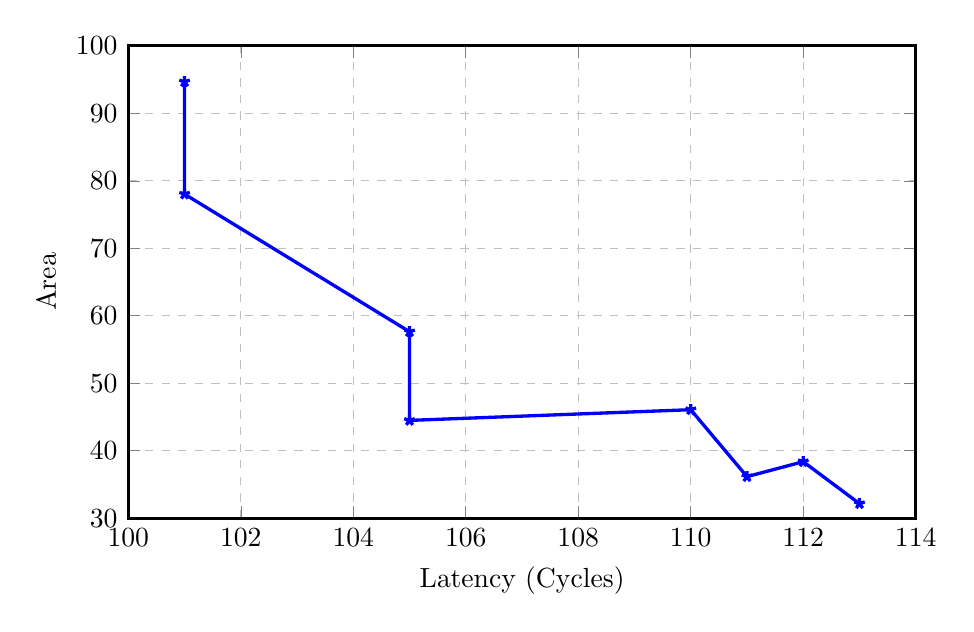
\begin{tikzpicture}
\begin{axis}[
scale only axis,
height=6cm,
width=10cm,
    xlabel={Latency (Cycles)},
    ylabel={Area},
    xmin=100, xmax=114,
    ymin=30, ymax=100,
    xtick={100,102,104,106,108,110,112,114},
    ytick={30,40,50,60,70,80,90,100},
    legend pos=north east,
    ymajorgrids=true,
    xmajorgrids=true,
    grid style=dashed,
    very thick
]
\addplot[
    color=blue,
    mark=star,
   % smooth
    ]
    coordinates {
    (101,94.675)(101,78.025)(105,57.6375)(105,44.495)(110,46.08)(111,36.165)(112,38.375)(113,32.166)
    };
\end{axis}
\end{tikzpicture}
\caption{Area Vs. Latency Curve for 4-Point FFT Implementation}
\label{plot_4fft}
\end{figure}